\documentclass{article}
% if you need to pass options to natbib, use, e.g.:
%     \PassOptionsToPackage{numbers, compress}{natbib}
% before loading neurips_2019

% ready for submission
% \usepackage{neurips_2019}

% to compile a preprint version, e.g., for submission to arXiv, add add the
% [preprint] option:
     \usepackage[preprint]{neurips_2019}
% to compile a camera-ready version, add the [final] option, e.g.:
     %\usepackage[final]{neurips_2019}

% to avoid loading the natbib package, add option nonatbib:
%     \usepackage[nonatbib]{neurips_2019}

\usepackage[utf8]{inputenc} % allow utf-8 input
\usepackage[T1]{fontenc}    % use 8-bit T1 fonts
\usepackage{hyperref}       % hyperlinks
\usepackage{url}            % simple URL typesetting
\usepackage{booktabs}       % professional-quality tables
\usepackage{amsfonts}       % blackboard math symbols
\usepackage{nicefrac}       % compact symbols for 1/2, etc.
\usepackage{microtype}      % microtypography
\usepackage{natbib}

\usepackage{graphicx}
\usepackage{subcaption}

\title{A model for evaluating physician performance}
\author{%
  Xiao Yang \\
  Department of Mathematics\\
  Carleton University\\
  Ottawa, ON, K1S 5B6 \\
  \texttt{barnettyang@cmail.carleton.ca} \\
  % examples of more authors
\And
Panxi Chen\\
 Department of Statistics \\
 University of Michigan Ann Arbor \\
 Ann Arbor, MI 48109-1107 \\
 \texttt{pxchen@umich.edu} \\
}

\begin{document}

\maketitle

\begin{abstract}
Since the last century, many efforts have been spent developing the ability of a health care
system, focusing on patients in the intensive care unit (ICU). Traditionally physicians participate
in 360 evaluations by answering questions scoring from 1 to 5, but this method fails to
incorporate patient information and thus can be biased. Assessment of physicians performance
depends on various factors such as professional knowledge level and behaviour competence,
therefore, we seek to develop a new model that includes patient information to evaluate
physician performance.
\end{abstract}

\section{Background}
  Patients admitted to the ICU are the most complex in the health care system often requiring expensive lifesaving technologies such as invasive monitoring, intubation and mechanical ventilation \cite{Jacobs}. Further, care within an intensive care unit is provided by a collaborative team of health professionals, including nurses, respiratory therapists, pharmacists, and physiotherapists. \\

  Many efforts have been made to develop ICU metrics to reflect the performance of a healthcare system. One definition of a physician's clinical performance (PCP) is the quantitative assessment of physician performance based on the rates at which their patients experience certain outcomes of care and the rates at which physicians adhere to evidence-based processes of care during their actual practice of medicine \cite{Street}. \\
  
  Traditionally, physicians participate in performance evaluations that are called 360 evaluations. The 360 model of feedback utilizes information from self-assessment, colleagues, non-physicians and patients. These assessments are useful, but fail to consider additional sources of data such as patient outcomes including ICU or hospital length of stay, complications, and mortality. There auxiliary information may provide a more encompassing picture of physician performance.  \\
  
  We are interested in developing a model for assessing the performance of an individual physician. Performance is a confluence of professional knowledge and behavioural competence. 

\section{Data set}

\subsection{physician data}
In physician's dataset, each physician had 360 feedback evaluations completed anonymously by a random sample of allied health professionals working in the ICU, and peer physicians including medical directors, physicians from non-critical care disciplines. Questions are from 7 domains: Medical Expert, Communicator, Leader, Advocate, Professional, Scholar, and Collaborator. Each question was scored on a 5-points scale.\\ 

Physician characteristics available included age, medical discipline and one attribute records if the physician is an administrative leader, or education leader in the university. \\

\subsection{patient data}

Each patient has a unique ID, the doctor who treated them and categorical variables that determine whether they are over 60, alive or dead after the treatment. 

APACHE II is an ICU-specific acuity of illness score calculated at the time of ICU admission based on the derangement of 12 physiological variables. The SOFA (Sepsis-associated organ failure assessment) score was developed by an expert consensus panel to describe the severity of organ failure at and following ICU admission. In addition, SOFA was designed to complement the acuity of illness score. \cite{Lambden} Both of the scores are considered useful to track patient status when they enter the ICU. The original data collected records SOFA score every day, until the patient is dead or leave the ICU. 


\section{Method}
We modified the 360 evaluation data set,filtering all incomplete rows and separate all evaluation questions to behavioural questions and professional questions, each yielding an average score for every physician. 

In the doctor data, we combine characters of doctor and 360 evaluation, and select overall score, evaluation rank, position, and summarize score from 360 evaluation to technical, non technical and overall scores. In the patient data frame,max/initial/end score for each physician by each patient are included along with the alive outcome, Apache II score and whether the patient is over 60.\\

We are mainly interested in the minimum, maximum and ending SOFA score of a given patient as they reflect the severity to reduce bias. Next we incorporate the Apache II, SOFA scores into this data frame. We now have a patient and a physician data frame at disposal. 

  After we cleaned and selected the important columns of our data, we proceed to apply machine learning techniques to predict whether a patient can survive, assigning different physicians. The output is a single value of 0 or 1, indicating death or alive after the treatment. 


\subsection{Naive KNN}

The result of KNN prediction \cite{KNN} is extremely bad, only with an accuracy around 0.411. Such low accuracy may be the consequence of the non-linearity of high-dimensionality of the data. The situation of each patient is unique, with few common traits, such as same symptoms or length of stay in ICU. The disparate cases prevents us from adopting a cluster technique. Thus, more thorough method is needed to replace the naive KNN.  
  
\subsection{Classification Tree}

Using the variable 'alive outcome', the classification tree \cite{BreimanL} shows 4 splits while the CP is set to default as 0.01. We find the optimal size of the tree by exploring the smallest 'x error', then the result shows that up to $71\%$ patients are predicted to be alive. The classification tree yields an overall training error of $0.31893$, and test error of $0.34515$.

\begin{figure}[h!]
  \centering
  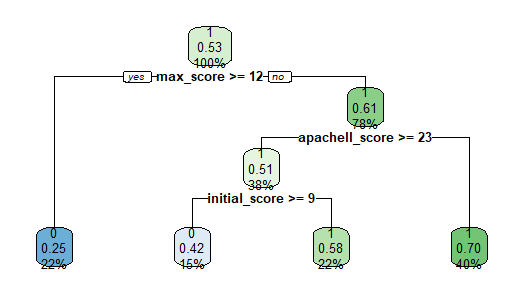
\includegraphics[width=120mm]{classificationTree.png}
  \caption{Classification Tree}
  \label{fig:Classification Tree output}
\end{figure}

\subsection{Random Forest}

A more complex model is random forest, which always performs the best overall \cite{Breiman}. But from the parameter we chose, training error is a lot better than that of classification tree, while test error is a little worse. The output from random forests suggests the five most important variables to predict a patient status, based on two different method, gini and accuracy. 

\begin{figure}[h!]
  \centering
  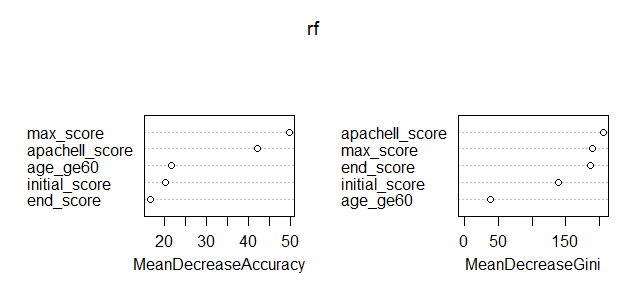
\includegraphics[width=120mm]{rf.png}
  \caption{Random Forest}
  \label{fig:Random Forest output}
\end{figure}


\subsection{PCA}

By standardizing the data, the first two components of PCA \cite{Mishra} could explain about $89\%$ of the data, and the scree plot suggests choosing the fist two components will suffice.\\

The biggest value in loading form for Apache II score is $0.533$ in the fourth component, which means if other scores the two patients give, are the same except their Apache II score, they differ the most when projected onto the PC 4 direction. \\ 

PC1 suggests initial score and max score are the two most important contributors, end score has fewer effect, all variables are positively correlated to the component;  
PC2 indicates end score is the most important contributor, while max score is the least important contributor.  \\

A larger emphasis on PC1 and smaller emphasis on PC2 leads to an overall well established presentation; A large emphasis on both PC1 and PC2 means great effect at the beginning and then gradually decreases; A small emphasis on both PC1 and PC2 is the contrary; the representation performs badly at first, but can improve later on.\\

From the plot of projections of data, we can see the distribution of the two classification from variable 'alive outcome'. A result of 'Alive' has more outliers, while 'Dead' are more tied together.

The bi-plot shows clearly that Apache II score and initial score are more correlated with smaller angle, which can be seen as a cluster.


\begin{figure}[htp] 
    \centering
    \subfloat[PCA plot]{%
        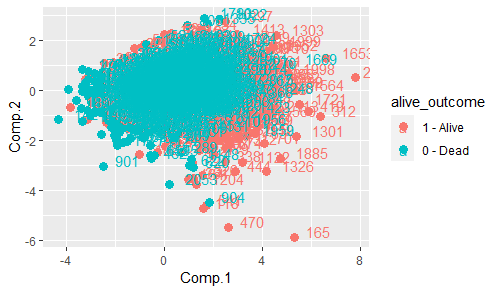
\includegraphics[width=0.4\textwidth]{ggpcaplot.png}%
        \label{fig:a}
%
        }%
    \hfill%
    \subfloat[Biplot]{%
        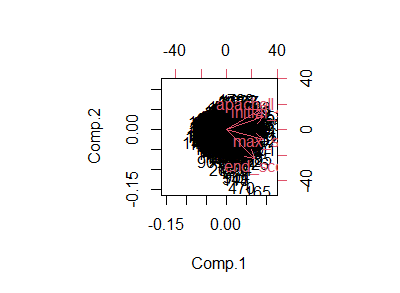
\includegraphics[width=0.4\textwidth]{biplot.png}%
        \label{fig:b}

        %
        }%
\end{figure}


\subsection{DMS}

The most similar pairs and the most dissimilar pairs are doctor 1 and doctor 15, respectively. For the most dissimilar pairs, the patient of doctor 1 is greater than 60 years old and is not alive at the end, but he gives very high score from the beginning to the end. \\

Perform MDS using above measure and plot the resulting projection into 2-d, so the two dimensions could preserve the real distance, then we can see which doctors are similar or dissimilar easily, with alive outcome noted by different color. From the plot, the two outcomes are clearly separated.\\

\begin{figure}[h!]
  \centering
  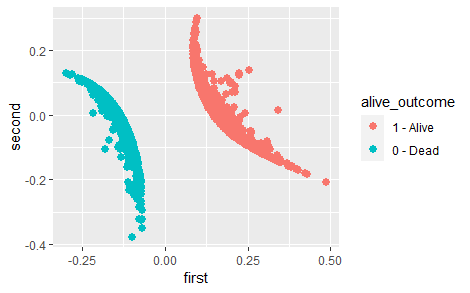
\includegraphics[width=100mm]{dms.png}
  \caption{DMS}
  \label{fig:DMS output}
\end{figure}

\section{Results}

By exploration data analysis, whether the patient is over 60 may affect the death rate. We split the patient data (after data cleaning) and sample $80\%$ of it as training data with the rest of them as test data. \\

A naive KNN yields the best k equals to 4 with accuracy $0.89$. Classification tree approach gives us the optimal size of $3$ with the smallest error 0.7646 with 3 splits. Random forest model shows that the most important variable is maximum SOFA score,which indicates the peak severity, followed by Apache II score. End score is also very important for Gini. \\

The scores of patients who are finally dead are more concentrated while the scores from alive patients are unstable and have outliers, indicated by PCA. We take the first two principle components which explain about $89\%$ data. From its bi-plot, we can see that the Apache II score is correlated to initial SOFA score, and maximum/end SOFA score do not have a correlation with Apache II score. Finally, by DMS we found that the scores of physicians have no overlap by separation of whether alive or not.

\section{Conclusion}

We developed a machine learning model that predicts whether a given patient will survive, assigning to a particular physician. From our analysis, we can conclude whether a patient is alive after treatment can significantly affect the score of the physician.\\

In particular, the 'alive outcome' variable is the most influential factor to a physicians' score, but most of the time, we can only forecast with a $70\%$ correct rate. Also, the average scores on 360 evaluation which contains professional knowledge and behavioural competence score do not have large impact on the 'alive outcome'. As a result, the reserve of professional knowledge is not the necessary condition to save the patient. Another observation that worth mentioning is that whether the patient is above 60 years old has a direct effect on death rates, corresponding to the common sense. Future work will include analysis of categorical variables, such as further distinguishing whether the physician is bedside or non-bedside to refine our model.

\section{Acknowledgement}

This study is from an open case challenge, hosted by Statistical Society of Canada. As part of the annual meeting in 2022, participants have access to the provided original data sets. Panxi implement the methods and provided insightful analysis of model output, while Xiao provides the main idea, with model framework, and is responsible for the rest work of paper. Both have equal contribution. The R code script and html output for better visualization are posted on github: \url{https://github.com/Barnett888/A-model-for-physician-evaluation}

\bigskip
\bigskip
\bigskip
\bigskip
\bigskip
\bigskip
\bigskip
\bigskip
\bigskip
\bigskip
\bigskip
\bigskip
\bigskip
\bigskip
\bigskip
\bigskip
\bigskip
\bigskip
\bigskip





\bibliography{references}{}
\bibliographystyle{plain}



\end{document}
